%=================================================================
\documentclass[informatics,article,submit,moreauthors]{Definitions/mdpi} 
%\documentclass[preprints,article,submit,moreauthors]{Definitions/mdpi} 
% For posting an early version of this manuscript as a preprint, you may use "preprints" as the journal. Changing "submit" to "accept" before posting will remove line numbers.

% Below journals will use APA reference format:
% admsci, aieduc, behavsci, businesses, econometrics, economies, education, ejihpe, famsci, games, humans, ijcs, ijfs, investment, fclam, jintelligence, journalmedia, jrfm, jsam, languages, opermanag, peacestud, pmh, psycholint, publications, tourismhosp, youth

% Below journals will use Chicago reference format:


%=================================================================
% MDPI internal commands - do not modify
\firstpage{1} 
\makeatletter 
\setcounter{page}{\@firstpage} 
\makeatother
\pubvolume{1}
\issuenum{1}
\articlenumber{0}
\pubyear{2026}
\copyrightyear{2026}
%\externaleditor{Firstname Lastname}
\datereceived{ } 
\daterevised{ }
\dateaccepted{ } 
\datepublished{ } 
%\datecorrected{}
%\dateretracted{}
%\doinum{}
%\pdfoutput=1
%\CorrStatement{yes}
%\longauthorlist{yes}
%\IsAssociation{yes}

%=================================================================
% Custom packages and macros for this manuscript
%=================================================================
\usepackage[ruled,vlined,linesnumbered]{algorithm2e}
%
\usepackage[T1]{fontenc}
% T1 fonts will be used to generate the final print and online PDFs,
% so please use T1 fonts in your manuscript whenever possible.
% Other font encondings may result in incorrect characters.
%
%\usepackage{graphicx}
%\usepackage{cite}
\usepackage{amsmath,amssymb,amsfonts}
\usepackage{graphicx}
\usepackage{subcaption}
\usepackage{booktabs}
\usepackage{multirow}
\usepackage{array}
\usepackage{tabularx}

\usepackage{textcomp}
\usepackage{xcolor}
\usepackage{url}
\usepackage{balance}
\usepackage{enumitem}
%\usepackage{hyperref}
\usepackage{tikz}
\usetikzlibrary{arrows.meta,fit,positioning}
%\usetikzlibrary{positioning}

\definecolor{authorange}{rgb}{0.75,0.42,0.0}
\newcommand{\expnote}[1]{\par\noindent{\small\color{red}$\blacktriangleright$
\textbf{[EXPERIMENT --- MKE]} \textit{#1}}\par}
\newcommand{\authnote}[1]{\par\noindent{\small\color{authorange}$\blacktriangleright$
\textbf{[AUTHORS]} \textit{#1}}\par}
% \renewcommand{\expnote}[1]{}   % <-- uncomment both to hide all notes
% \renewcommand{\authnote}[1]{}



%=================================================================
% Please use the following mathematics environments: Theorem, Lemma, Corollary, Proposition, Characterization, Property, Problem, Example, ExamplesandDefinitions, Hypothesis, Remark, Definition, Notation, Assumption
%% For proofs, please use the proof environment (the amsthm package is loaded by the MDPI class).

%=================================================================
% Full title of the paper (Capitalized)
\Title{Reducing Trace-Complexity Bias in Microservice Anomaly Scoring via Weighted Residual Service Trace Vectors}

% Author Orchid ID: enter ID or remove command
%\newcommand{\orcidauthorA}{} 
\newcommand{\orcidauthorB}{0000-0002-9029-2187} 


% Authors, for the paper (add full first names)
\Author{Pavan Kumar Ramina $^{1}$\orcidA{}, and Murali Krishna Enduri $^{1,}$*\orcidB{}}

%\longauthorlist{yes}

% MDPI internal command: Authors, for metadata in PDF
\AuthorNames{Pavan Kumar Ramina and Murali Krishna Enduri}

%\longauthorlist{yes}

% Affiliations / Addresses (Add [1] after \address if there is only one affiliation.)
\address{%
$^{1}$ \quad
Department of Computer Science and Engineering, SRM University-AP, Amaravati 522 240, Andhra Pradesh, India; muralikrishna.e@srmap.edu.in}

% Contact information of the corresponding author
\corres{Correspondence: muralikrishna.e@srmap.edu.in}
 
\abstract{Distributed trace anomaly scoring commonly represents each trace as a
	Service Trace Vector (STV), where features correspond to service call
	paths and values encode latency. However, raw STV-based scoring can be
	strongly influenced by trace structural complexity. In this paper, we
	show empirically on three TrainTicket configurations of
	\texttt{ts-order-service} that baseline STV~+~Isolation Forest scores
	correlate strongly with trace size, with correlations of approximately
	\(r=0.85\)--\(0.98\) for span and service-count based complexity
	measures. We propose WR-STV, a lightweight STV-based anomaly scoring
	method that replaces raw feature scoring with clipped standardized
	residuals, applies log-frequency reliability weighting, and aggregates
	the top-\(k\) weighted residual contributors into a trace-level score.
	On held-out non-injected traces, WR-STV reduces the measured
	score-complexity correlation from approximately \(r=0.87\) to
	\(r=0.30\). Under controlled STV-visible latency injection, WR-STV
	improves within-dataset ROC-AUC from \(0.605\) to \(0.814\), with
	random-visible injection used to test whether the improvement depends
	on perturbing only high-duration spans. Additional baseline comparisons
	indicate that residual normalization accounts for most of the gain,
	while reliability weighting provides a smaller, metric-dependent
	refinement. WR-STV also provides interpretable service-path-level
	evidence and lightweight per-trace scoring. The evaluation is scoped to
	synthetic latency perturbations on three configurations of one
	benchmark service.}

% Keywords
\keyword{Microservices; Distributed Tracing;  Anomaly Detection; Service Trace Vector; Residual Normalization;  Trace Complexity Bias; Explainability.} 

% The fields PACS, MSC, and JEL may be left empty or commented out if not applicable
%\PACS{J0101}
%\MSC{05C69; 05C85; 05C76; 05C25; 68R10}
%\JEL{}

%%%%%%%%%%%%%%%%%%%%%%%%%%%%%%%%%%%%%%%%%%
\begin{document}


\section{Introduction}
\label{sec:introduction}

% ------------------------------------------------------------
% Paragraph 1 -- Background: microservices + distributed tracing
% ------------------------------------------------------------
Microservice architectures decompose large applications into collections of independently deployed services that communicate through networked requests  \cite{dragoni2017microservices}. Although this design improves scalability, modularity, and deployment flexibility, it also complicates performance diagnosis because a single user request may traverse many services and generate a distributed execution path. Distributed tracing systems record this execution as a trace composed of spans, where each span captures a service operation, timing information, and parent-child relationships \cite{sigelman2010dapper}. As microservice systems scale, manual inspection of traces becomes impractical, creating a need for automated methods that can identify traces whose execution deviates from expected behavior and guide operators toward likely sources of latency or failure.

% ------------------------------------------------------------
% Paragraph 2 -- Why trace anomaly detection matters
% ------------------------------------------------------------
At the scale of modern microservice deployment, distributed tracing
frameworks continuously collect large volumes of execution traces,
making manual inspection challenging for human operators. Early
industrial approaches often relied on manually maintained rules,
including service-specific return-code rules, to identify abnormal
executions. As services evolve, however, these rules require continual
maintenance because the meaning and usage of service-specific return
codes may change over time, reducing their long-term effectiveness
\cite{liu2020traceanomaly}. These challenges have motivated
learning-based trace anomaly detection methods that model the
characteristics of normal trace executions and automatically identify
traces whose behavior deviates from the learned patterns, allowing
operators to prioritize investigation without continually redesigning
rule sets. 
% ------------------------------------------------------------
% Paragraph 3 -- Existing methods and the STV representation
% ------------------------------------------------------------
Learning-based trace anomaly detection depends heavily on how
distributed traces are represented for machine learning. Previous
studies have explored execution sequences, graph-based models,
learned embeddings, and fixed-dimensional vector representations \cite{liu2020traceanomaly,zhang2022deeptralog,xie2023tracevae}. Among these, the Service Trace Vector (STV), introduced in
TraceAnomaly \cite{liu2020traceanomaly}, transforms variable-length
distributed traces into fixed-dimensional feature vectors suitable for
machine learning. In an STV, each feature corresponds to a specific
service reached through a particular call path, while its value
represents a latency-related characteristic associated with that
service path (Section~\ref{sec:background}). Because every feature has
a direct correspondence to an actual service path, STVs preserve
service-level interpretability while providing a compact numerical
representation of distributed traces. Furthermore, because STVs are
fixed-dimensional feature vectors, they can be analyzed using a wide
range of conventional statistical and machine learning techniques,
making them a flexible representation for trace anomaly detection.
However, the effectiveness of such approaches depends not only on the
trace representation itself, but also on how anomaly scores are
derived from the resulting feature vectors.Existing STV- and graph-based approaches have demonstrated strong anomaly detection performance across several benchmark microservice datasets. However, comparatively little attention has been given to understanding whether the anomaly scores produced by these methods are influenced by intrinsic structural properties of traces, such as execution size or call-path complexity.


% ------------------------------------------------------------
% Paragraph 4 -- The research gap: complexity bias
% ------------------------------------------------------------
We identify a systematic weakness in STV-based anomaly scoring: when an STV
is scored using a generic unsupervised detector trained directly on raw,
unnormalized feature values, the resulting anomaly score can become
strongly influenced by trace \emph{size}, independent of trace
\emph{health}. To better understand this phenomenon, we analyze real, non-injected
test traces from three configuration variants of the
\texttt{ts-order-service} microservice in the TrainTicket benchmark \cite{zhou2021trainticket}.
Across these datasets, the Pearson correlation between baseline
STV~+~Isolation Forest anomaly scores and the number of distinct
services ranges from $r = 0.968$ to $0.982$, while the correlation with
the number of spans ranges from $r = 0.854$ to $0.981$
(Table~\ref{tab:complexity-bias-baseline}). Because these measurements are obtained from traces without injected
anomalies, the observed correlations cannot be explained by successful
detection of synthetic faults. Instead, they indicate that the structural characteristics of a trace can
substantially influence anomaly scores even when the observed executions
are operationally normal. This suggests that anomaly scoring based solely on raw STV feature
values may find it more difficult to distinguish genuinely abnormal
executions from structurally complex but otherwise normal traces.
% ------------------------------------------------------------
% Paragraph 5 -- Proposed method
% ------------------------------------------------------------
We propose \textbf{WR-STV} (Weighted Residual Service Trace Vector), which
replaces the raw STV value at each feature with a standardized residual
against that feature's learned training-time mean and variance, clips the
residual for numerical stability, weights it by a log-frequency reliability
term that down-weights rarely observed paths, and scores the trace by the
mean of its top-$k$ weighted absolute residuals. This keeps the
representation's per-service-path interpretability while reducing its dependence on trace size (Section~\ref{sec:methodology}).

% ------------------------------------------------------------
% Contributions
% ------------------------------------------------------------
The main contributions of this paper are:

\begin{itemize}
	\item \textbf{An empirical demonstration of trace-complexity bias} in
	STV~+~Isolation Forest anomaly scoring, measured directly on real,
	non-injected test traces from three TrainTicket configurations
	($r \approx 0.85$--$0.98$ with baseline score; reduced to
	$r \approx 0.24$--$0.30$ under WR-STV).
	
	\item \textbf{Weighted Residual Service Trace Vectors}: a lightweight residual-standardization and
	reliability-weighting scheme for STV scoring, together with an ablation
	study isolating how much of its improvement comes from standardization versus
	weighting.
	
	\item \textbf{A controlled, circularity-checked evaluation}: evaluate WR-STV using latency
	anomalies injected into both the largest-duration visible span and a randomly chosen visible span (robustness check), injection-strength sensitivity, classical  anomaly detection baselines, and cross-dataset transfer across all six directed train/test pairs. Showing that WR-STV's detection improvement is not an artifact of always targeting the feature to which its scoring function is most sensitive.
	
	
	\item \textbf{Quantitative interpretability and failure analysis}:
	top-$k$ explanation overlap against known injected paths, and a
	taxonomy of the conditions under which WR-STV fails to rank an injected
	trace above its original.
\end{itemize}


%%%%%%%%%%%%%%%%%%%%%%%%% Section 2 %%%%%%%%%%%%%%%%%%%%%%%%%%%%%%%%%%

\section{Related Work}
\label{sec:related-work}

\subsection{Distributed Trace Representations}

The effectiveness of learning-based trace anomaly detection depends
strongly on how distributed traces are represented before analysis.
Distributed traces are variable-length execution records with service
invocation paths, parent-child relationships, and heterogeneous latency
behavior. Prior work has therefore explored several representations for
trace analysis. TraceAnomaly represents each trace as a fixed-dimensional
Service Trace Vector (STV), where features correspond to service call
paths and values encode latency-related behavior~\cite{liu2020traceanomaly}.
Graph-based approaches instead preserve more of the trace topology.
DeepTraLog constructs a trace event graph that combines invocation
structure with log events~\cite{zhang2022deeptralog}, while TraceVAE
models microservice traces using a graph variational autoencoder
designed for tree-structured trace data~\cite{xie2023tracevae}. Other
recent approaches incorporate additional telemetry such as profiling
metrics or resource utilization to enrich trace representations
\cite{panahandeh2024serviceanomaly,alomari2025contextaware}.

These representations involve different trade-offs. Fixed-dimensional
vectors such as STVs are lightweight and directly interpretable because
each feature maps to a concrete service path, but they may collapse
structural information. Graph-based and multi-modal models preserve more
execution structure and operational context, but typically require more
complex learning architectures and may reduce transparency of individual
feature contributions. Our work builds on the interpretability and
simplicity of STVs, but studies a different question: whether anomaly
scores derived from raw STV features are systematically influenced by
trace structural complexity.

\subsection{Trace-Based Anomaly Detection and Localization}

Early approaches to microservice anomaly detection often relied on
manually defined rules or service-specific heuristics to identify
abnormal executions~\cite{liu2020traceanomaly}. As microservice systems
increased in scale and complexity, these rule-based techniques became
harder to maintain, motivating learning-based methods that model normal
trace behavior directly from data. TraceAnomaly learns the distribution
of normal STVs using service-level deep Bayesian networks and assigns
higher anomaly scores to traces that deviate from the learned normal
behavior~\cite{liu2020traceanomaly}. Because STV features correspond to
service paths, this representation also provides service-path-level
diagnostic information.

Subsequent methods improve trace anomaly detection by using richer
representations or more expressive models. DeepTraLog combines trace and
log information in a graph neural architecture with a deep support vector
data description objective~\cite{zhang2022deeptralog}. TraceGra uses
graph deep learning to model trace-based anomaly detection in
microservice systems~\cite{chen2023tracegra}. ServiceAnomaly combines
distributed traces with profiling metrics in an annotated graph to
detect abnormal microservice executions~\cite{panahandeh2024serviceanomaly}.
Recent work has also explored context-aware trace graph embeddings and
resource-metric autoencoders for anomaly detection and localization
\cite{alomari2025contextaware,xing2025multidim}.

These methods primarily focus on improving anomaly detection accuracy,
capturing a richer trace structure, or enhancing fault localization. In
contrast, our work focuses on the behavior of the anomaly scoring process
itself. Specifically, we examine whether STV-based anomaly scores can be
biased by structural properties of traces, such as the number of spans or
services, even when the traces are operationally normal.

\subsection{Research Gap: Bias in STV-Based Anomaly Scoring}

Existing trace anomaly detection studies have advanced the state of the
art through improved trace representations, graph neural architectures,
deep generative models, and multi-modal telemetry fusion. However, they
typically evaluate detection accuracy or localization quality, while the
relationship between anomaly score and trace structural complexity is
rarely examined directly. This leaves open an important question for
STV-based anomaly scoring: does a high anomaly score reflect abnormal
service-path behavior, or can it also reflect the fact that a trace is
structurally larger than other traces?

To the best of our knowledge, prior STV-based trace anomaly detection
studies have not explicitly quantified whether raw STV anomaly scores
are correlated with trace-complexity measures such as span count and
service count. Our work addresses this gap by measuring the dependency
directly, proposing a lightweight residual scoring method designed to
reduce it, and evaluating the resulting effect on both trace-complexity
bias and controlled latency-anomaly scoring performance.

%%%%%%%%%%%%%%%%%%%%%% Section 3 %%%%%%%%%%%%%%%%%%%%%%%%%%%%%

\section{Background and Motivation}
\label{sec:background}

\subsection{Distributed Traces}

A distributed trace records the end-to-end execution of a single user
request as it propagates through multiple interacting microservices
\cite{sigelman2010dapper}. Each trace consists of a collection of
\emph{spans}, where every span represents an individual service
invocation together with execution metadata, including the service name,
operation name, start time, duration, and parent-child relationship. The
parent-child relationships among spans allow a trace to be interpreted as
a causal execution structure, from which request paths across services
can be reconstructed. Because traces vary in both execution path and
structural complexity, they provide a rich source of information for
performance analysis and anomaly detection.

\subsection{Service Trace Vectors}

Although distributed traces capture detailed execution behavior, their
variable length and hierarchical structure make them unsuitable for
direct use by conventional machine learning algorithms that require
fixed-dimensional inputs. TraceAnomaly~\cite{liu2020traceanomaly}
addresses this limitation through the Service Trace Vector (STV), which
maps each distributed trace into a fixed-dimensional feature vector while
preserving the correspondence between features and service call paths.

Following TraceAnomaly, each feature 
$j=(\mathrm{service},\mathrm{service\_path})$ corresponds to a unique service reached through a particular root-to-node execution path observed during training.
For a trace \(i\), the feature value is defined as

\begin{equation}
	x_{i,j}=\log\!\left(1+d_{i,j}\right),
	\label{eq:stv-value}
\end{equation}

where \(d_{i,j}\) denotes the maximum observed duration for feature \(j\)
within trace \(i\). When the same service-path feature appears multiple
times in a trace, the maximum duration is retained. Features that are
absent from a trace are assigned a sentinel value of \(-1\), indicating
that the corresponding service path was not executed. The logarithmic
transformation reduces the dynamic range of span durations while
preserving their relative ordering. Because every feature corresponds to
a specific service path, the resulting representation remains directly
interpretable and enables anomaly scores to be associated with concrete
execution paths rather than latent embedding dimensions.

\subsection{Motivation: Trace-Complexity Bias}
\label{sec:complexity-bias-background}

The STV representation provides an interpretable numerical description
of distributed traces, but it also introduces an important
characteristic: structurally larger traces naturally populate more STV
features than smaller traces. Consequently, traces containing more
services or spans may appear more unusual to an anomaly scoring method,
even when the underlying system behavior is operationally normal.

To investigate whether this structural difference influences anomaly
scoring, we analyze the relationship between baseline STV anomaly scores
and two measures of trace complexity: the number of distinct services
and the total number of spans contained in each trace. The analysis is
performed on real, non-injected test traces collected from three
TrainTicket configurations~\cite{zhou2021trainticket}.

\begin{table}[t]
	\centering
	\caption{Pearson correlation between baseline STV~+~Isolation Forest anomaly
		score and trace-complexity metrics (real, non-injected traces).}
	\label{tab:complexity-bias-baseline}
	\begin{tabular}{lccc}
		\toprule
		& \textbf{Dataset 1} & \textbf{Dataset 2} & \textbf{Dataset 3} \\
		\midrule
		num\_services      & 0.977 & 0.982 & 0.968 \\
		num\_spans         & 0.854 & 0.981 & 0.975 \\
		total\_duration    & 0.605 & 0.698 & 0.672 \\
		max\_span\_duration & 0.550 & 0.627 & 0.681 \\
		mean\_span\_duration & 0.035 & $-$0.034 & 0.089 \\
		\bottomrule
	\end{tabular}
\end{table}


As shown in Table~\ref{tab:complexity-bias-baseline}, baseline anomaly
scores exhibit consistently strong positive correlations with both
complexity measures across all three datasets. Because these
measurements are obtained from traces without injected anomalies, the
observed correlations cannot be attributed to successful detection of
synthetic faults. Instead, they indicate that structural properties of a
trace can substantially influence anomaly scores even when the observed
executions are operationally normal.

Figure~\ref{fig:bias} visualizes this relationship by plotting baseline
anomaly scores against trace size for real, non-injected traces. The
overall trend demonstrates that larger traces tend to receive higher
baseline anomaly scores, motivating the need for an anomaly scoring
strategy that is less sensitive to structural complexity.

\begin{figure*}[t]
	\centering
	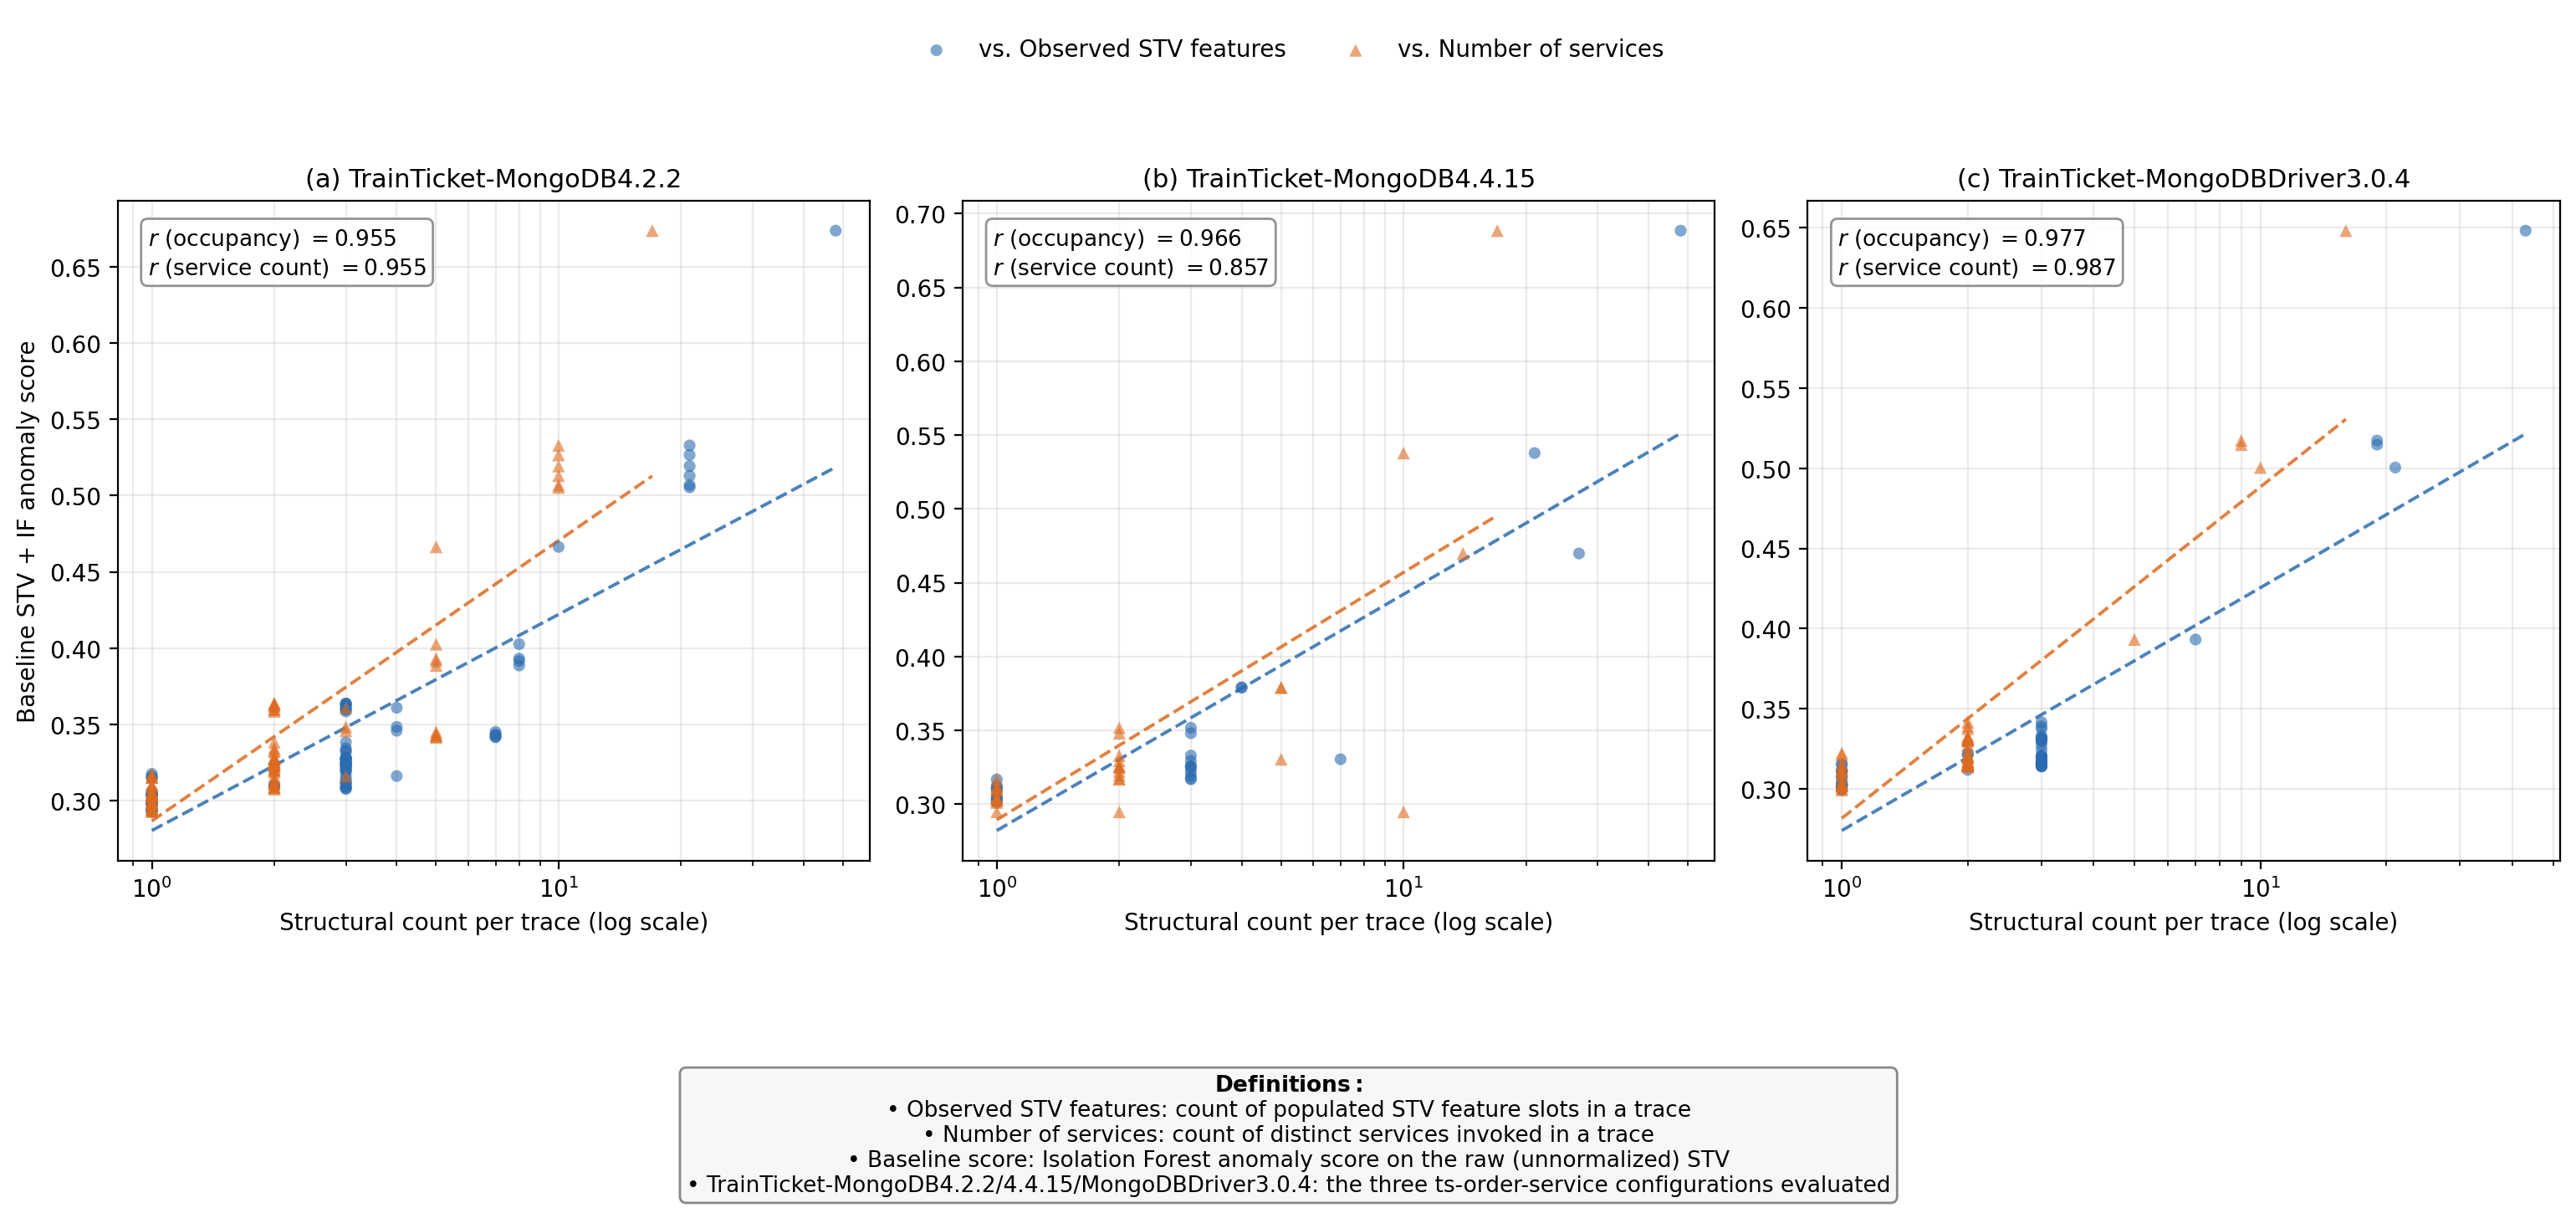
\includegraphics[width=\textwidth]{complexity_bias_scatter.png}
	\caption{Baseline STV anomaly score versus trace complexity on real,
		non-injected traces from three TrainTicket configurations. Each point
		represents one trace. The observed positive correlations indicate that
		structurally larger traces tend to receive higher baseline anomaly
		scores even in the absence of injected anomalies.}
	\label{fig:bias}
\end{figure*}

\subsection{Design Intuition}

The observations above suggest that anomaly scoring should depend on how
unusual each feature is relative to its own expected behavior rather
than on its absolute magnitude alone. Features whose latency values are
consistent with their historical behavior should contribute little to the
final anomaly score, even when they occur in a large trace. In contrast,
features exhibiting unusually large deviations from their own learned
normal behavior should receive greater emphasis. This intuition motivates
the Weighted Residual Service Trace Vector (WR-STV) method introduced in
the next section, which preserves the interpretability of the original
STV representation while reducing the influence of trace structural
complexity on anomaly scoring.

%%%%%%%%%%%%%%%%%%Section 3 %%%%%%%%%%%%%%%%%%%%%%%%%%
\section{Proposed Method}
\label{sec:methodology}

\subsection{Overview}

WR-STV is an STV-based anomaly scoring framework that transforms raw
service-path latency features into reliability-weighted residual
contributions. The method computes an anomaly score for each trace in
five stages, all derived from statistics learned from the training split
only: (1) construct the baseline Service Trace Vector (STV), (2) compute
per-feature training statistics, (3) convert observed values into
clipped standardized residuals, (4) weight each residual by a reliability
term reflecting how often that feature was observed during training, and
(5) aggregate the top-\(k\) weighted residuals into a single trace-level
score. Fig.~\ref{fig:pipeline} summarizes the full pipeline.

\begin{figure*}[t]
	\centering
	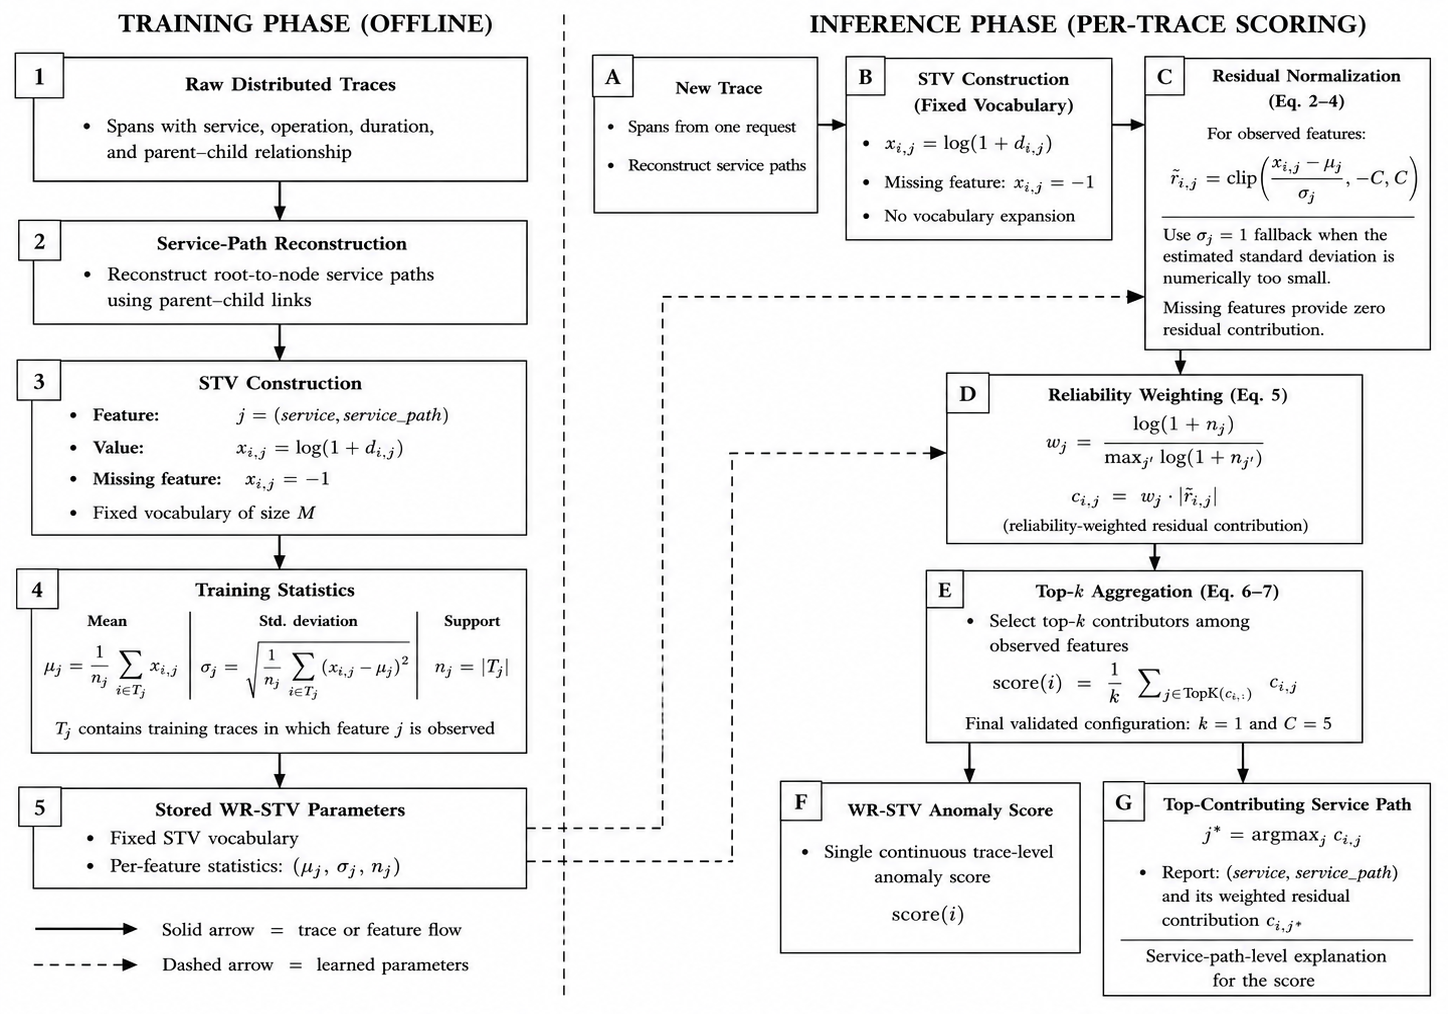
\includegraphics[width=\textwidth]{wrstv_pipeline.png}
	\caption{Overview of the WR-STV anomaly scoring pipeline. Feature
		statistics and reliability weights are learned from training traces
		only and applied to each test trace using a fixed STV vocabulary.
		Top-\(k\) weighted residual aggregation produces a trace-level
		anomaly score and service-path-level explanatory evidence.}
	\label{fig:pipeline}
\end{figure*}

Given a distributed trace, WR-STV produces a single anomaly score that
quantifies the degree to which the trace deviates from the statistical
behavior learned from training traces. Rather than modifying the
underlying trace representation, WR-STV retains the original STV
representation and instead modifies the anomaly scoring process through
feature-wise residual standardization, reliability weighting, and
top-\(k\) aggregation. This design preserves the interpretability of STV
features while reducing the influence of trace structural complexity on
the final anomaly score.


\subsection{Service Trace Vector Construction}

Following the Service Trace Vector (STV) representation introduced by
TraceAnomaly~\cite{liu2020traceanomaly}, each trace is mapped to a
fixed-vocabulary vector, where feature
\(j=(\text{service},\text{service\_path})\) is valued by
\(x_{i,j}=\log(1+d_{i,j})\). A sentinel value of \(-1\) is used when
feature \(j\) is not observed in trace \(i\). The feature vocabulary and
all statistics described in the following subsections are learned
exclusively from the training split. During inference, the same
vocabulary is reused without modification, and service paths not observed
during training are treated as absent rather than added as new features.
Using a fixed vocabulary ensures that training and inference operate over
a consistent feature space.

\subsection{Residual Normalization}

Raw STV values are not directly comparable across service-path features
because different paths naturally exhibit different latency scales and
variability. WR-STV therefore normalizes each observed feature relative
to its own training-time behavior. For each feature \(j\), we compute
the training-time mean and standard deviation over the training traces in
which \(j\) is observed:

\begin{align}
	\mu_j
	&=
	\frac{1}{n_j}
	\sum_{i \in \mathcal{T}_j}
	x_{i,j},
	\label{eq:mean}
	\\
	\sigma_j
	&=
	\sqrt{
		\frac{1}{n_j}
		\sum_{i \in \mathcal{T}_j}
		(x_{i,j} - \mu_j)^2
	},
	\label{eq:std}
\end{align}

\noindent where \(\mathcal{T}_j\) is the set of training traces in which
feature \(j\) is present and \(n_j = |\mathcal{T}_j|\). If a feature has
insufficient observations or a numerically small standard deviation, the
implementation uses a unit standard deviation fallback to avoid unstable
division.

For an observed value \(x_{i,j}\) at inference time, the clipped
standardized residual is

\begin{equation}
	\tilde{r}_{i,j}
	=
	\operatorname{clip}
	\left(
	\frac{x_{i,j}-\mu_j}{\sigma_j},
	-C,
	C
	\right),
	\label{eq:residual}
\end{equation}

\noindent where \(C\) denotes the residual clipping threshold. The
clipping operation improves numerical stability for features with very
small standard deviations and prevents individual feature deviations from
disproportionately influencing the final anomaly score. Features absent
from a trace are assigned zero residual contribution and therefore do not
increase the anomaly score.

\subsection{Reliability Weighting}

Features observed infrequently during training provide fewer samples for
estimating their underlying latency distribution, resulting in greater
uncertainty in the estimated mean and standard deviation. Consequently,
standardized residuals associated with such features are more susceptible
to sampling variability. To reduce the influence of these uncertain
estimates, each feature is assigned a reliability weight based on its
training-time observation frequency:

\begin{equation}
	w_j
	=
	\frac{\log(1+n_j)}
	{\max_{j'} \log(1+n_{j'})}.
	\label{eq:weight}
\end{equation}

\noindent The logarithmic transformation compresses large count
differences while preserving the ordering of feature support. Thus,
\(w_j \in (0,1]\), with the most frequently observed feature receiving
weight \(1\). Features observed more frequently during training receive
larger weights, whereas infrequently observed features are down-weighted,
reducing their influence on the final anomaly score.

\subsection{Top-\(k\) Weighted Residual Scoring}

The weighted contribution of feature \(j\) in trace \(i\) is defined as

\begin{equation}
	c_{i,j}
	=
	w_j
	\left|
	\tilde{r}_{i,j}
	\right|.
	\label{eq:contribution}
\end{equation}

\noindent Larger standardized deviations from learned normal behavior
produce larger contributions, moderated by the feature reliability
weight.

Rather than summing all feature contributions, which can reintroduce
dependence on the number of populated features in a trace, WR-STV
aggregates only the strongest residual evidence. The final anomaly score
is computed as the average of the \(k\) largest weighted contributions:

\begin{equation}
	\operatorname{score}(i)
	=
	\frac{1}{k}
	\sum_{j \in \operatorname{Top}_k(c_{i,:})}
	c_{i,j}.
	\label{eq:topk}
\end{equation}

\noindent This aggregation emphasizes the most significant service-path
deviations while limiting the influence of numerous low-magnitude
residuals that are unlikely to indicate anomalous behavior. The value of
\(k\) is selected through validation, as described in
Section~\ref{sec:hyperparameter-selection}. In the final configuration,
we use \(k=1\). Under this setting, the anomaly score corresponds to the
largest weighted residual within the trace, and the associated
service-path feature is reported as the explanation for the score in the
interpretability analysis presented in
Section~\ref{sec:results-explainability}.

\subsection{Request-Aware Calibration (Ablation Variant)}

As an ablation study, we also evaluate a request-aware variant in which
the statistics in Equations~\ref{eq:mean}--\ref{eq:std} are computed
separately for each root operation when sufficient training samples are
available. When insufficient data exist for a particular request type,
the corresponding global statistics are used instead.

Although this variant further reduces the observed correlation between
anomaly score and trace complexity
\begin{table}[t]
	\centering
	\caption{Complexity-bias correlation across methods, averaged over
		num\_services and num\_spans (real, non-injected test traces). This is the
		paper's central bias-reduction evidence.}
	\label{tab:complexity-bias-all-methods}
	\begin{tabular}{lcc}
		\toprule
		\textbf{Method} & \textbf{corr.\ num\_services} & \textbf{corr.\ num\_spans} \\
		\midrule
		Baseline STV + IF                 & 0.868 & 0.820 \\
		Enhanced STV + IF                 & 0.835 & 0.779 \\
		Global Residual STV (unweighted)  & 0.383 & 0.324 \\
		\textbf{WR-STV (weighted)}        & \textbf{0.296} & \textbf{0.238} \\
		Request-Aware WR-STV              & 0.274 & 0.218 \\
		\bottomrule
	\end{tabular}
\end{table}
(Table~\ref{tab:complexity-bias-all-methods}), it does not consistently improve
anomaly scoring performance. Therefore, we report it as an ablation
rather than the primary WR-STV method.



\section{Experimental Setup}
\label{sec:experimental-setup}

\subsection{Datasets}

We evaluate WR-STV using three trace sets collected from the
TrainTicket benchmark microservice system~\cite{zhou2021trainticket}.
Each trace set corresponds to a distinct configuration of
\texttt{ts-order-service}:
\texttt{ts-order-service\_mongodb\_4.2.2},
\texttt{ts-order-service\_mongodb\_4.4.15}, and
\texttt{ts-order-service\_3.0.4-mongodb-driver}. We refer to these
configurations as Dataset~1, Dataset~2, and Dataset~3, respectively.
TrainTicket is a benchmark microservice system designed for fault
analysis and debugging studies, making it suitable for controlled
experiments on microservice observability and anomaly scoring.

The three configurations vary the service version and MongoDB driver
while preserving broadly similar service-level functionality. This makes
them useful for both within-dataset evaluation and cross-dataset transfer
analysis. In particular, the related but non-identical configurations
allow us to study how WR-STV behaves when training and test traces share
similar service structures but differ in observed latency distributions
and service-path coverage.

Table~\ref{tab:dataset-stats} summarizes trace, span, and service
counts, along with trace-graph quality checks performed before modeling.
Across all three datasets, each trace contains exactly one root span, no
non-root span has a missing parent, and no duplicate
\((\text{traceID}, \text{spanID})\) pairs are present.

\begin{table}[t]
	\centering
	\caption{Dataset statistics and trace-graph quality checks.}
	\label{tab:dataset-stats}
	\begin{tabular}{lccc}
		\toprule
		& \textbf{Dataset 1} & \textbf{Dataset 2} & \textbf{Dataset 3} \\
		\midrule
		Traces          & 269 & 86  & 160 \\
		Spans           & 3{,}788 & 1{,}306 & 1{,}993 \\
		Distinct services & 32 & 33 & 33 \\
		\midrule
		Exactly 1 root span/trace & \checkmark & \checkmark & \checkmark \\
		Non-root spans w/ missing parent & 0 & 0 & 0 \\
		Duplicate (traceID, spanID) pairs & 0 & 0 & 0 \\
		\bottomrule
	\end{tabular}
\end{table}


\subsection{Preprocessing Pipeline}

Spans are grouped by trace identifier, and each span's root-to-node
service path is reconstructed by following parent-child relationships
from the trace root. Following Equation~\ref{eq:stv-value}, spans that
share the same \((\text{service}, \text{service\_path})\) feature within
a single trace are aggregated into one STV feature by retaining the
maximum observed duration. We use maximum aggregation because the slowest
occurrence of a repeated service path is often the most actionable signal
for latency anomaly triage, whereas mean aggregation may dilute localized
delays.

For every experimental split, the STV vocabulary, feature-wise
normalization statistics, and reliability weights are estimated only from
the training traces. The learned vocabulary and statistics are then
applied unchanged to validation and test traces. This protocol prevents
test-set leakage and ensures that unseen service paths at inference time
are treated as absent rather than being used to expand the feature space.

\subsection{Synthetic Latency Injection}

Because the trace sets do not provide per-trace ground-truth anomaly
labels, we evaluate anomaly scoring using controlled synthetic latency
injection. For a normal test trace, an injected copy is created by
multiplying the duration of selected STV-visible spans by an injection
factor \(f\). A span is considered STV-visible if its
\((\text{service}, \text{service\_path})\) feature appears in the
training vocabulary. The original trace is assigned label \(0\), while
the injected copy is assigned label \(1\).

We evaluate two span-selection strategies:

\begin{itemize}
	\item \textbf{Largest-visible injection:} selects up to \(m\)
	STV-visible spans with the largest original durations. This is the
	primary controlled latency-injection setting.
	
	\item \textbf{Random-visible injection:} selects up to \(m\)
	STV-visible spans uniformly at random, regardless of original
	duration. This setting tests whether WR-STV's advantage depends on
	always perturbing high-duration spans.
\end{itemize}

Unless otherwise specified, experiments use \(f=30\) and \(m=3\). We
also perform injection-strength sensitivity analysis using
\(f \in \{5,10,20,30\}\), as reported in
Section~\ref{sec:results-sensitivity}. Both injection strategies are
restricted to STV-visible dimensions, meaning that they evaluate
controlled latency deviations on service paths already observed during
training. This is a deliberate scope limitation and is discussed further
in Section~\ref{sec:threats}.

\subsection{Baseline Methods}

We compare WR-STV against both raw-STV and residual-STV baselines:

\begin{itemize}
	\item \textbf{Baseline STV + Isolation Forest:} the raw STV
	representation from Equation~\ref{eq:stv-value}, without feature
	normalization, scored using Isolation Forest~\cite{liu2008iforest}.
	This is the primary baseline used to measure trace-complexity bias.
	
	\item \textbf{Enhanced STV + Isolation Forest:} z-score-normalized
	residual features from Equations~\ref{eq:mean}--\ref{eq:residual},
	scored using Isolation Forest. This baseline isolates the effect of
	residual normalization independent of WR-STV's top-\(k\) scoring
	rule and reliability weighting.
	
	\item \textbf{Max-Z Residual STV:} the maximum absolute residual from
	Equation~\ref{eq:residual}, using \(k=1\) and no reliability
	weighting. This isolates the contribution of the reliability weight
	in Equation~\ref{eq:weight}.
	
	\item \textbf{Top-3 Residual STV:} the mean of the top three
	unweighted absolute residuals. This tests whether aggregating
	multiple residual contributors changes ranking performance without
	reliability weighting.
	
	\item \textbf{Residual STV + LOF / One-Class SVM:} the standardized
	residual representation scored using Local Outlier Factor
	\cite{breunig2000lof} and One-Class SVM~\cite{scholkopf2001ocsvm}.
	This compares WR-STV's simple top-\(k\) aggregation against classical
	detectors applied to the same residual feature space.
	
	\item \textbf{Raw STV + LOF / One-Class SVM:} the same two detectors
	applied directly to the unnormalized STV representation. This tests
	whether the behavior observed with Isolation Forest is specific to
	one detector family or also appears under other classical
	unsupervised methods.
\end{itemize}

\subsection{Evaluation Metrics}

We report ROC-AUC, average precision (AUPRC), F1 at an oracle threshold,
precision@\(N_+\), and pairwise win rate. Here, \(N_+\) denotes the
number of injected traces in an evaluation split. The oracle-threshold
F1 is computed by labeling the top \(N_+\) scored traces as anomalous and
is therefore used only as a ranking diagnostic, not as a deployment-ready
thresholding result.

Pairwise win rate is computed over matched
\((\text{original}, \text{injected})\) trace pairs. A pair is counted as a
win when the injected trace receives a strictly higher anomaly score than
its corresponding original trace. This metric directly measures whether
a scoring method ranks a controlled latency perturbation above the normal
trace from which it was generated.

\subsection{Hyperparameter Selection}
\label{sec:hyperparameter-selection}

The WR-STV top-\(k\) parameter and residual clip bound \(C\) are selected
using an inner validation split. We search over
\(k \in \{1,3,5\}\) and \(C \in \{3.0,5.0,10.0\}\). The validation split
is drawn from the outer training set, with \(30\%\) of the outer training
traces reserved for validation. Test traces are not used during
hyperparameter selection. This procedure selects \(k=1\) and \(C=5.0\),
which are used for all final WR-STV results.

\begin{table}[t]
	\centering
	\caption{Hyperparameter selection on a held-out validation split
		(independent of all test-set metrics reported elsewhere in this paper).}
	\label{tab:hyperparam-validation}
	\begin{tabular}{lc}
		\toprule
		\textbf{Hyperparameter} & \textbf{Selected value} \\
		\midrule
		$k$ (top-$k$ features aggregated) & 1 \\
		$C$ (residual clip bound)         & 5.0 \\
		\bottomrule
	\end{tabular}
	
	\vspace{4pt}
	\footnotesize
\end{table}


\subsection{Implementation Details}

All experiments are implemented in Python using NumPy, pandas, and
scikit-learn. Isolation Forest uses 200 estimators in all experiments.
Local Outlier Factor is evaluated in novelty-detection mode, and
One-Class SVM uses the radial-basis-function kernel with
\(\nu=0.1\) and \(\gamma=\texttt{scale}\). Unless otherwise specified,
each dataset is split 65:35 into training and test traces. The split is performed uniformly at random at the trace level using the specified random seed, ensuring that individual traces appear in only one partition. Within-dataset
experiments are repeated over five random seeds for each dataset,
resulting in \(3 \times 5 = 15\) runs.

The overall experimental protocol is as follows. First, STVs are
constructed from the training split, and the training vocabulary is fixed.
Second, WR-STV feature statistics and reliability weights are estimated
from the same training split only. Third, the fitted scoring procedure is
applied unchanged to held-out validation or test traces. Finally,
synthetic latency anomalies are injected only into evaluation traces, and
metrics are computed over the resulting normal-vs-injected trace pairs.

\section{Results and Discussion}
\label{sec:results}

\subsection{RQ1: Does Trace-Complexity Bias Exist?}

The baseline results indicate that trace-complexity bias is substantial.
Table~\ref{tab:complexity-bias-baseline} shows that anomaly scores
produced by the baseline STV representation combined with Isolation
Forest are strongly correlated with trace structural complexity. Across
the three datasets, the Pearson correlation between anomaly score and
the number of services ranges from \(r=0.968\) to \(0.982\), while the
correlation with the number of spans ranges from \(r=0.854\) to
\(0.981\). These consistently high correlations indicate that
structurally larger traces receive systematically higher anomaly scores
even in the absence of injected anomalies. This demonstrates that trace
complexity introduces a substantial bias into the baseline anomaly
scoring process and provides the primary motivation for WR-STV.

\subsection{RQ2: Does Residual Normalization Reduce It?}

\begin{table}[t]
	\centering
	\caption{Complexity-bias correlation across methods, averaged over
		num\_services and num\_spans (real, non-injected test traces). This is the
		paper's central bias-reduction evidence.}
	\label{tab:complexity-bias-all-methods}
	\begin{tabular}{lcc}
		\toprule
		\textbf{Method} & \textbf{corr.\ num\_services} & \textbf{corr.\ num\_spans} \\
		\midrule
		Baseline STV + IF                 & 0.868 & 0.820 \\
		Enhanced STV + IF                 & 0.835 & 0.779 \\
		Global Residual STV (unweighted)  & 0.383 & 0.324 \\
		\textbf{WR-STV (weighted)}        & \textbf{0.296} & \textbf{0.238} \\
		Request-Aware WR-STV              & 0.274 & 0.218 \\
		\bottomrule
	\end{tabular}
\end{table}
Residual normalization substantially reduces, but does not eliminate,
trace-complexity bias. Table~\ref{tab:complexity-bias-all-methods} shows that
WR-STV considerably reduces the dependence of anomaly scores on trace
structural complexity. Averaged across datasets and seeds, the Pearson
correlation with the number of services decreases from \(r=0.868\)
under the baseline detector to \(r=0.296\) using WR-STV and further to
\(r=0.274\) under the request-aware variant. Similarly, the correlation
with the number of spans decreases from \(r=0.820\) to \(r=0.238\) and
\(r=0.218\), respectively.

The remaining positive correlation is expected because larger traces
naturally provide more opportunities for at least one extreme feature
residual to occur. Consequently, WR-STV should be interpreted as
substantially reducing, rather than completely removing,
trace-complexity bias while preserving sensitivity to path-visible
latency deviations.

\subsection{RQ3: Does WR-STV Improve Anomaly Scoring and How Does It Compare with Baselines?}
\label{sec:results-main}

\begin{table}[t]
	\centering
	\caption{Main detection results: baseline vs.\ WR-STV, largest-visible
		injection ($f=30$, $m=3$), mean over datasets/seeds.}
	\label{tab:main-results}
	\begin{tabular}{lccc}
		\toprule
		& \textbf{ROC-AUC} & \textbf{AUPRC} & \textbf{F1} \\
		\midrule
		\multicolumn{4}{l}{\textit{Within-dataset}} \\
		Baseline STV + IF & 0.605 & 0.574 & 0.583 \\
		\textbf{WR-STV ($k$=1, $C$=5)} & \textbf{0.814} & \textbf{0.812} & \textbf{0.738} \\
		\midrule
		\multicolumn{4}{l}{\textit{Cross-dataset (6 directed pairs)}} \\
		Baseline STV + IF & 0.622 & 0.573 & 0.602 \\
		\textbf{WR-STV ($k$=1, $C$=5)} & \textbf{0.803} & \textbf{0.804} & \textbf{0.722} \\
		\bottomrule
	\end{tabular}
\end{table}
\begin{table}[t]
	\centering
	\caption{Paired statistical tests, WR-STV vs.\ baseline STV~+~IF.}
	\label{tab:main-stats}
	\begin{tabular}{lcccc}
		\toprule
		& \textbf{Gain} & \textbf{Cohen's $d_z$} & \textbf{paired-$t$ $p$} & \textbf{Wilcoxon $p$} \\
		\midrule
		\multicolumn{5}{l}{\textit{Within-dataset (n=15 seed$\times$dataset rows)}} \\
		ROC-AUC & +0.209 & 2.78 & $3.68 \times 10^{-8}$ & $6.1 \times 10^{-5}$ \\
		AUPRC   & +0.237 & 3.79 & $6.87 \times 10^{-10}$ & $6.1 \times 10^{-5}$ \\
		F1      & +0.155 & 2.70 & $5.34 \times 10^{-8}$ & $9.82 \times 10^{-4}$ \\
		\midrule
		\multicolumn{5}{l}{\textit{Cross-dataset (n=6 directed pairs)}} \\
		ROC-AUC & +0.182 & 1.92 & $0.0053$ & $0.03125$ \\
		AUPRC   & +0.231 & 2.67 & $0.00126$ & $0.03125$ \\
		F1      & +0.120 & 1.69 & $0.00893$ & $0.03125$ \\
		\bottomrule
	\end{tabular}
\end{table}


Table~\ref{tab:main-results} and Table~\ref{tab:main-stats} report the
primary anomaly scoring comparison. Compared with baseline STV +
Isolation Forest, WR-STV improves the within-dataset ROC-AUC from
\(0.605\) to \(0.814\). The cross-dataset ROC-AUC also improves from
\(0.622\) to \(0.803\). The within-dataset improvement is statistically
significant with a large paired effect size. The cross-dataset
comparison also shows a large paired effect, although its statistical
interpretation is limited by the small number of directed train-test
pairs.

These results indicate that the primary performance improvement arises
from feature-wise residual normalization rather than from replacing one
unsupervised detector with another. Standardizing each service-path
feature relative to its learned latency distribution produces a scoring
space that is substantially less influenced by trace structural
complexity, allowing latency deviations to be identified more
consistently across heterogeneous traces. The ablation results should
be interpreted as evidence for residual normalization as the primary
component: the additional reliability weighting is metric-dependent
and is not statistically significant for ROC-AUC or F1 in the reported
comparison. The reported $p$-values are exploratory and are not
adjusted for the multiple comparisons across metrics, methods, and
transfer pairs.
\begin{table}[t]
	\centering
	\caption{Detection performance vs.\ classical baselines, random-visible
		injection ($f=30$), mean ROC-AUC.}
	\label{tab:extra-baselines}
	\begin{tabular}{lc}
		\toprule
		\textbf{Method} & \textbf{ROC-AUC} \\
		\midrule
		\textbf{WR-STV ($k$=1, $C$=5)}   & \textbf{0.811} \\
		Max-Z Residual STV (unweighted) & 0.798 \\
		Residual STV + LOF              & 0.785 \\
		Residual STV + One-Class SVM    & 0.775 \\
		Top-3 Residual STV (unweighted) & 0.771 \\
		Raw STV + One-Class SVM         & 0.761 \\
		Raw STV + LOF                   & 0.707 \\
		Enhanced STV + IF               & 0.673 \\
		Baseline STV + IF               & 0.604 \\
		\bottomrule
	\end{tabular}
\end{table}

\begin{table}[t]
	\centering
	\caption{Paired significance, WR-STV vs.\ its two closest competitors
		(random-visible injection). Report both rows -- the non-significant
		ROC-AUC/F1 comparison against the unweighted variant is an honest and
		important ablation finding, not a result to omit.}
	\label{tab:extra-baseline-stats}
	\begin{tabular}{lccc}
		\toprule
		\textbf{Comparison} & \textbf{Metric} & \textbf{Diff.} & \textbf{$p$ (paired-$t$ / Wilcoxon)} \\
		\midrule
		\multirow{3}{*}{vs.\ Max-Z Residual STV}
		& ROC-AUC & $+0.013$ & $0.108$ / $0.135$ \\
		& AUPRC   & $+0.065$ & $5.1\times10^{-5}$ / -- \\
		& F1      & $+0.003$ & $0.735$ / -- \\
		\midrule
		\multirow{2}{*}{vs.\ Residual STV + LOF}
		& ROC-AUC & $+0.025$ & $0.0026$ / -- \\
		& F1      & $+0.007$ & $0.32$ / -- \\
		\bottomrule
	\end{tabular}
\end{table}


Table~\ref{tab:extra-baselines} further compares WR-STV with classical
baselines operating on the same residual representation. Although WR-STV
achieves the highest overall ROC-AUC (\(0.811\)), the margin over the
unweighted Max-Z Residual STV (\(0.798\)) is relatively small.

Table~\ref{tab:extra-baselines} shows that this difference is not
statistically significant for ROC-AUC (\(p=0.108\)) or F1
(\(p=0.735\)), while only Average Precision reaches statistical
significance. This suggests that most of WR-STV's performance gain
originates from residual normalization, whereas reliability weighting
provides a smaller, metric-dependent incremental improvement.

\subsection{RQ4: How Robust Is WR-STV to Injection Strength?}
\label{sec:results-sensitivity}

\begin{figure}[t]
    \centering
    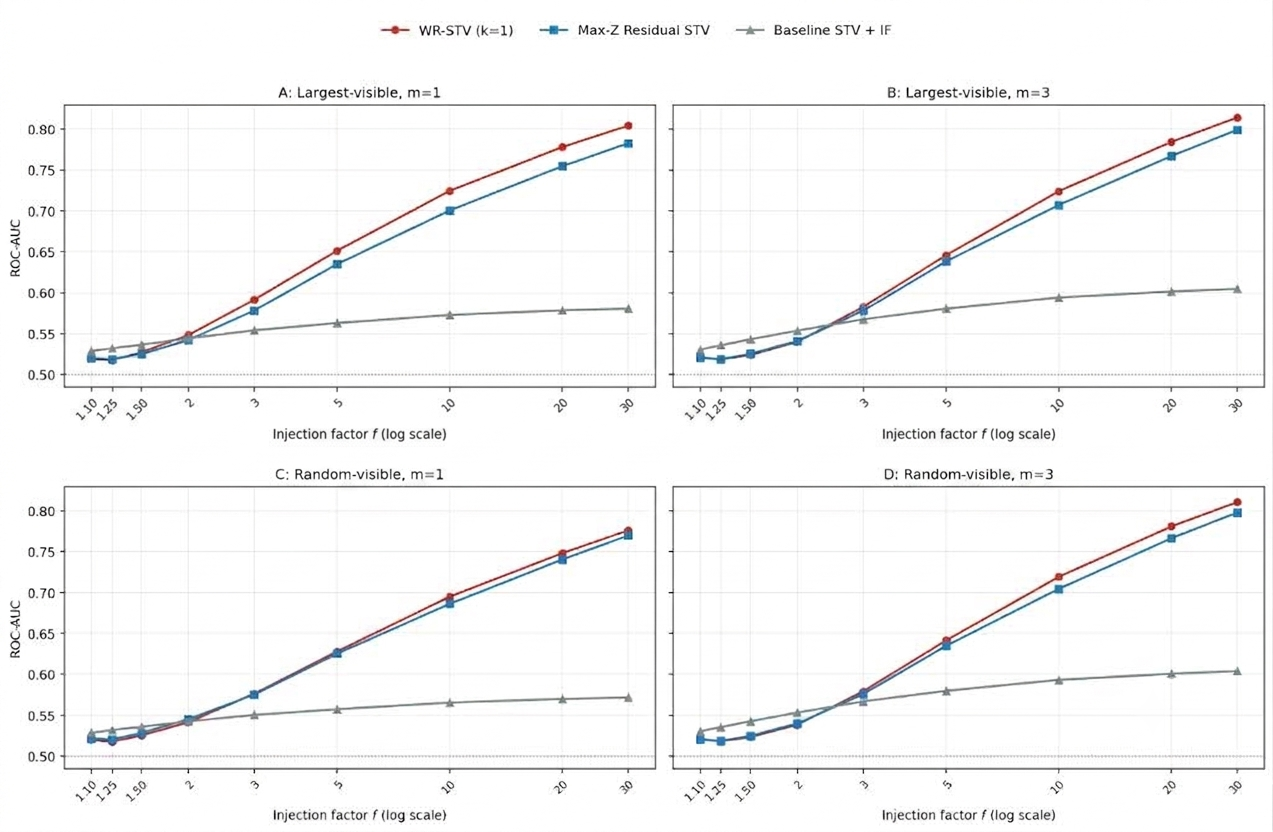
\includegraphics[width=0.85\linewidth]{fig_sensitivity.png}
    \caption{Sensitivity to injection strength $f$ (largest-visible strategy), WR-STV vs.\ baseline}
    \label{fig:sensitivity}
\end{figure}
	
	
	
Figure~\ref{fig:sensitivity} shows that WR-STV's ROC-AUC, AUPRC, and F1
increase monotonically as the injection factor increases from
\(5\times\) to \(30\times\), while baseline STV~+~IF is comparatively
insensitive to injection strength over the same range. This indicates
that WR-STV's score responds to the magnitude of controlled latency
deviations, which is desirable for an anomaly scoring method. However,
even the smallest evaluated factor, \(5\times\), represents a large
multiplicative latency deviation. These results therefore demonstrate
sensitivity trends under controlled perturbations rather than
performance under subtle production-scale degradations.

We additionally evaluate the random-visible injection strategy, which
selects injected spans uniformly at random among STV-visible spans rather
than always selecting the largest-duration visible span. This checks
whether WR-STV's advantage is an artifact of injections always landing
on spans most likely to affect a top-residual scoring rule. WR-STV's
ROC-AUC changes negligibly between strategies
(\(0.814 \rightarrow 0.811\)), as does the baseline's
(\(0.605 \rightarrow 0.604\)). This indicates that the observed
advantage is not explained by this specific form of injection
circularity. Nevertheless, both strategies remain restricted to
STV-visible service paths and model only multiplicative latency
anomalies, limitations discussed further in Section~\ref{sec:threats}.

\subsection{RQ5: Does WR-STV Generalize Across Datasets?}
\begin{table}[t]
	\centering
	\caption{WR-STV cross-dataset transfer, all six directed train$\rightarrow$test
		pairs (largest-visible injection)}.
	\label{tab:cross-pairs}
	\begin{tabular}{lccc}
		\toprule
		\textbf{Train $\rightarrow$ Test} & \textbf{ROC-AUC} & \textbf{AUPRC} & \textbf{F1} \\
		\midrule
		Dataset 1 $\rightarrow$ Dataset 2 & 0.891 & 0.888 & 0.800 \\
		Dataset 1 $\rightarrow$ Dataset 3 & 0.891 & 0.892 & 0.796 \\
		Dataset 2 $\rightarrow$ Dataset 1 & 0.611 & 0.644 & 0.587 \\
		Dataset 2 $\rightarrow$ Dataset 3 & 0.790 & 0.789 & 0.680 \\
		Dataset 3 $\rightarrow$ Dataset 1 & 0.760 & 0.752 & 0.684 \\
		Dataset 3 $\rightarrow$ Dataset 2 & 0.872 & 0.861 & 0.785 \\
		\midrule
		\textbf{Mean (6 pairs)} & \textbf{0.803} & \textbf{0.804} & \textbf{0.722} \\
		\bottomrule
	\end{tabular}
\end{table}


Table~\ref{tab:cross-pairs} reports all six directed train--test pairs.
Transfer performance varies across pairs, with ROC-AUC ranging from
\(0.611\) to \(0.891\). The strongest transfer is observed for
Dataset~1~\(\rightarrow\)~Dataset~2 and Dataset~1~\(\rightarrow\)~Dataset~3
(both \(0.891\)), while the weakest transfer occurs for
Dataset~2~\(\rightarrow\)~Dataset~1 (\(0.611\)). We checked whether this degradation is explained by
unseen service paths at test time and found that \(97.8\%\) of
test-trace STV-visible events were covered by the Dataset~2 training
vocabulary. This suggests that the weak transfer pair is not primarily a
coverage problem.
\begin{table}[t]
	\centering
	\caption{Latency distribution shift vs.\ cross-dataset transfer performance
		(shared STV-visible features between train and test).}
	\label{tab:distribution-shift}
	\begin{tabular}{lccc}
		\toprule
		\textbf{Train $\rightarrow$ Test} & \textbf{Wtd.\ mean Wasserstein} & \textbf{$p_{90}$ std.\ shift} & \textbf{ROC-AUC} \\
		\midrule
		Dataset 2 $\rightarrow$ Dataset 1 & 0.973 & 2.737 & 0.611 \\
		Dataset 1 $\rightarrow$ Dataset 3 & 0.872 & 1.515 & 0.891 \\
		Dataset 1 $\rightarrow$ Dataset 2 & 0.772 & 1.707 & 0.891 \\
		\bottomrule
	\end{tabular}
	
	\vspace{4pt}
	\footnotesize
	Spearman correlation ($p_{90}$ standardized shift vs.\ ROC-AUC, all 6
	directed pairs): $r = -0.829$, $p = 0.0416$. \textbf{Report as exploratory}
	-- $n=6$ pairs are drawn from only 3 underlying datasets and are not
	independent samples; do not present this $p$-value as confirmatory.
\end{table}

Table~\ref{tab:distribution-shift} instead shows that this pair has the
largest latency distribution shift on shared features
(\(p_{90}\) standardized shift \(=2.74\), compared with
\(\leq 1.71\) for the stronger pairs shown). The exploratory correlation
across all six directed pairs (Spearman \(r=-0.83\), \(n=6\)) is more
consistent with distribution shift than with vocabulary coverage as an
explanation for transfer degradation. This suggests that successful
cross-dataset transfer may depend more strongly on preserving the
latency distributions of shared service paths than on maintaining
identical feature vocabularies. Since this conclusion is based on only
six directed transfer pairs, it should be regarded as exploratory rather
than definitive.

\subsection{RQ6: Can WR-STV Explain Anomalies?}
\label{sec:results-explainability}
\begin{table}[t]
	\centering
	\caption{WR-STV explanation overlap against known injected paths
		(aggregate cross-dataset, largest-visible injection).}
	\label{tab:explainability}
	\begin{tabular}{lcc}
		\toprule
		\textbf{Top-$k$} & \textbf{Service overlap} & \textbf{Path overlap} \\
		\midrule
		Top-1  & 0.638 & 0.500 \\
		Top-3  & 0.937 & 0.915 \\
		Top-5  & 0.967 & 0.946 \\
		Top-10 & 0.998 & 0.992 \\
		\bottomrule
	\end{tabular}
\end{table}

Table~\ref{tab:explainability} shows that WR-STV's top-3 contributing
service paths recover the actual injected service paths with
\(93.7\%\) service overlap and \(91.4\%\) path overlap, aggregated across
all cross-dataset pairs. This result is conditional on the injected
anomaly being among the largest residual signals in the trace. The same
scoring mechanism used for anomaly scoring is also used for localization,
so this result should be interpreted as evidence that WR-STV can point to
anomalies it scores highly, not as an independently validated
localization capability for anomalies of unknown type.



\subsection{RQ7: Where Does WR-STV Fail?}
\begin{table}[t]
	\centering
	\caption{WR-STV failure taxonomy: cases where the injected trace did not
		score above its original (279 unique failures after deduplication from
		1{,}395 raw pairwise failure rows).}
	\label{tab:failure-categories}
	\begin{tabular}{lcc}
		\toprule
		\textbf{Category} & \textbf{Count} & \textbf{\%} \\
		\midrule
		Pre-existing high normal score       & 124 & 44.44 \\
		Very short trace, limited evidence   & 105 & 37.63 \\
		Score unchanged after injection      & 19  & 6.81 \\
		Low residual after injection         & 12  & 4.30 \\
		Uncategorized (distribution/ranking) & 10  & 3.58 \\
		Low reliability weight               & 5   & 1.79 \\
		High train-variance path             & 4   & 1.43 \\
		\bottomrule
	\end{tabular}
\end{table}
Table~\ref{tab:failure-categories} categorizes the 279 unique cases,
after deduplication from 1{,}395 raw pairwise rows, where WR-STV did not
rank an injected trace above its original. The two dominant categories,
pre-existing high normal score (\(44.4\%\)) and very short traces with
limited path evidence (\(37.6\%\), mean \(\approx 1.3\) spans), together
account for \(82\%\) of failures. Both categories have clear causal
interpretations: a trace that already scores in the upper tail of the
normal-score distribution has little room to be pushed higher by an
injected anomaly, and a one-or-two-span trace provides limited
STV-visible evidence for a top-\(k\) aggregation with \(k=1\).

These failure modes suggest that many WR-STV failures arise from limited
or unfavorable evidence available to the scorer rather than from random
instability of the scoring rule. In practice, traces with very few
observable service-path features may require confidence estimates,
abstention rules, or complementary detectors rather than being treated
as equally reliable scoring targets.

\subsection{RQ8: Is WR-STV Computationally Lightweight?}

Although computational efficiency is not the primary contribution of
this work, WR-STV also offers practical scoring advantages.
\begin{table}[t]
	\centering
	\caption{Runtime comparison, mean over datasets and seeds.}
	\label{tab:runtime}
	\begin{tabular}{lcc}
		\toprule
		\textbf{Method} & \textbf{Total (s)} & \textbf{Per-trace scoring (ms)} \\
		\midrule
		\textbf{WR-STV}    & \textbf{0.171} & \textbf{0.0238} \\
		Enhanced STV + IF  & 0.576 & 0.3627 \\
		Baseline STV + IF  & 0.607 & 0.3647 \\
		\bottomrule
	\end{tabular}
	WR-STV is $\approx$3.5$\times$ faster end-to-end and $\approx$15$\times$
	faster per-trace than Isolation Forest-based baselines. Memory footprint is
	negligible for all methods at this dataset scale and is not a
	differentiator; report it in one sentence in text, not as a table.
\end{table}
Table~\ref{tab:runtime} shows that WR-STV requires approximately
\(0.0238\)\,ms per trace, compared with approximately \(0.36\)\,ms for
Isolation Forest-based baselines, corresponding to roughly a
\(15\times\) reduction in scoring time. This improvement is expected
because WR-STV performs lightweight statistical computations using
precomputed feature statistics and avoids ensemble-tree inference during
deployment. Consequently, WR-STV has favorable computational properties
for high-throughput scoring scenarios, although full online deployment
would require additional thresholding and operational validation.

\subsection{Summary of Findings}

Across the evaluated research questions, the results support the central
hypothesis of this work. Raw STV representations scored with Isolation
Forest are strongly influenced by trace structural complexity. WR-STV
substantially reduces this dependence through feature-wise residual
normalization and improves controlled latency-anomaly ranking in
within-dataset experiments, with promising but more limited evidence for
cross-dataset transfer. The method also provides service-path-level
interpretability, predictable failure modes, and lightweight scoring
cost. Overall, the results support WR-STV as a bias-aware anomaly
scoring framework for controlled STV-visible latency deviations rather
than a general-purpose solution to all microservice anomaly types.


\section{Threats to Validity}
\label{sec:threats}

\subsection{Internal Validity}

The main internal validity risk is optimistic bias from design or
hyperparameter choices. To reduce this risk, the WR-STV top-\(k\)
parameter and residual clip bound \(C\) are selected using a validation
split independent of the held-out test traces, as described in
Section~\ref{sec:hyperparameter-selection}. The primary injection
setting \((f=30, m=3)\) is reported together with injection
strength sensitivity over \(f \in \{5,10,20,30\}\), so the effect of injection
strength is visible rather than hidden in a single operating point.
All STV vocabularies, residual statistics, and reliability weights are
estimated from training traces only and then applied unchanged to
validation or test traces.

\subsection{Construct Validity}

The evaluation measures controlled synthetic latency anomalies rather
than naturally occurring production failures. Injected anomalies are
created by multiplying selected span durations, so the evaluation
primarily tests sensitivity to path-visible latency deviations. It does
not test non-latency anomalies such as incorrect responses, missing
calls, dropped spans, novel service paths, or structural changes in the
trace graph. In addition, both largest-visible and random-visible
injection strategies are constrained to STV-visible service paths, i.e.,
features already present in the training vocabulary. Therefore, the
results characterize WR-STV under controlled STV-visible latency
perturbations rather than all possible microservice anomaly types.

The reported F1 score is computed using an oracle threshold that labels
the top \(N_+\) scored traces as anomalous, where \(N_+\) is the number
of injected traces in the evaluation split. This metric should be
interpreted as a ranking diagnostic rather than as expected deployment
precision or recall under an unknown operational threshold.

\subsection{External Validity}

The evaluation is limited to three configuration variants of
\texttt{ts-order-service} within the TrainTicket benchmark. Although
these configurations provide useful version-induced variation, they
represent a single benchmark system and a single target service. The
results may not generalize to other services, other microservice
benchmarks, production workloads, or environments with substantially
different tracing quality, traffic patterns, or service-call structures.
Additional evaluation on other services, benchmark systems, and real
production incident data is required before making broader
generalization claims.

\subsection{Statistical Conclusion Validity}

Within-dataset statistical analyses are based on repeated experiments
over five random seeds for each of three datasets, yielding \(n=15\)
seed-dataset runs. These repeated runs improve robustness to random
train-test splitting, but they are not equivalent to fifteen independent
datasets. Cross-dataset transfer analysis is even more limited: it uses
only six directed train-test pairs derived from the same three datasets.
Consequently, cross-dataset statistical tests should be interpreted as
exploratory evidence supporting observed trends rather than definitive
statistical confirmation.

\section{Conclusion }
\label{sec:conclusion}

This paper studied trace-complexity bias in a common microservice
anomaly scoring pattern: Service Trace Vector representations scored by
an unnormalized unsupervised detector. On real, non-injected TrainTicket
traces, baseline STV~+~Isolation Forest anomaly scores correlate strongly
with trace size, with correlations of approximately
\(r \approx 0.85\)--\(0.98\) for span and service-count based complexity
measures. This finding shows that raw STV-based scores can reflect trace
structural complexity rather than only operational abnormality.

To address this issue, we proposed WR-STV, a lightweight STV-based
scoring method that applies per-feature residual standardization,
residual clipping, reliability weighting, and top-\(k\) aggregation.
Across the evaluated datasets, WR-STV substantially reduces the measured
correlation between anomaly score and trace complexity
(\(r \approx 0.30\)) while improving controlled STV-visible latency
anomaly ranking over baseline STV~+~Isolation Forest
(within-dataset ROC-AUC \(0.605 \rightarrow 0.814\)). Cross-dataset
experiments show dataset-dependent transfer behavior, improving the
six-pair mean from \(0.622\) to \(0.803\), with pairwise ROC-AUC values
from $0.611$ to $0.891$. These results should be interpreted cautiously
because they are based on only six directed train-test pairs from one
benchmark service. In particular, Dataset~2~$\rightarrow$~Dataset~1
is weak ($0.611$), despite stronger transfer when Dataset~1 is the
training source.

The ablation results indicate that most of the improvement comes from
feature-wise residual normalization, while the proposed reliability
weighting contributes a smaller, metric-dependent refinement. WR-STV
also provides interpretable service-path-level evidence, with top-3
contributing service paths recovering more than \(90\%\) of known
injected paths in the evaluated setting. Runtime analysis further shows
that WR-STV achieves roughly a \(15\times\) lower per-trace scoring time
than Isolation Forest-based baselines. Overall, the results support
WR-STV as a lightweight and interpretable approach for reducing
trace-complexity bias in controlled STV-visible latency anomaly scoring,
rather than as a general solution to all microservice anomaly types.

Future work will extend this study in four directions: evaluating
anomalies beyond STV-visible latency perturbations (e.g., dropped calls,
novel call paths, missing spans, and other structural trace anomalies);
testing generalization of the complexity-bias pattern on additional
services, benchmark systems, and production-like traces beyond
\texttt{ts-order-service}; attaching confidence estimates or abstention
rules for very short, low-evidence traces, which the failure analysis
identifies as a predictable failure mode; and validating WR-STV against
real-world fault-injection or incident-labeled datasets to assess its
behavior on anomalies not generated by this paper's own evaluation
procedure.

%%%%%%%%%%%%%%%%%%%%%%%%%%%%%%%%%%%%%%%%%%%%%%%%%%%%%%%%%%%%

\authorcontributions{Conceptualization, P.K.R; methodology, P.K.R. and M.K.E; formal analysis, P.K.R.; investigation, M.K.E and P.K.R.; software, P.K.R.; validation, M.K.E.; data curation, M.K.E.; writing-original draft preparation, P.K.R and M.K.E.; writing-review and editing, P.K.R. and M.K.E.; visualization, M.K.E.; supervision, P.K.R.; project administration, P.K.R; funding acquisition, M. K. E. All authors have read and agreed to the published version of the manuscript.}

\funding{This work was financially supported by SRM University-AP, Andhra Pradesh, India. The authors gratefully acknowledge the financial support provided by the university.}

\dataavailability{The source code, data sets and reproduction scripts are openly available at \url{https://github.com/pVnpNdu02/Reducing-Trace-Complexity-Bias-WR-STV}.}



\section*{Disclosure of Generative AI Use}
During the preparation of this manuscript the authors used Claude (Anthropic) to assist with language assistance, LaTeX preparation, and verification code for the algorithm and experiments. The authors reviewed and edited the content and take full responsibility for the content of the publication.
\section*{Conflicts of Interest}
The authors declare no conflict of interest.

%
% ---- Bibliography ----
%
% BibTeX users should specify bibliography style 'splncs04'.
% References will then be sorted and formatted in the correct style.
%
%\bibliographystyle{splncs04}
\section*{References}
\bibliography{references}
\end{document}

